\chapter{Bildakquise und Datenaufbereitung}
Eine der grundlegenden Funktionalitäten des Projektes ist die Anzeige der Bilddaten des Ultraschallgerätes auf einem Smartphone Display. Dieser Prozess kann auf verschiedene Arten implementiert werden, welche unterschiedliche Vor- und Nachteile haben. Alle Ansätze haben jedoch eine grundlegende Abfolge von Arbeitsschritten gemein (siehe Abbildung \ref{fig:Bildakquise_schritte}).\\

\begin{figure}[h]
	\centering
	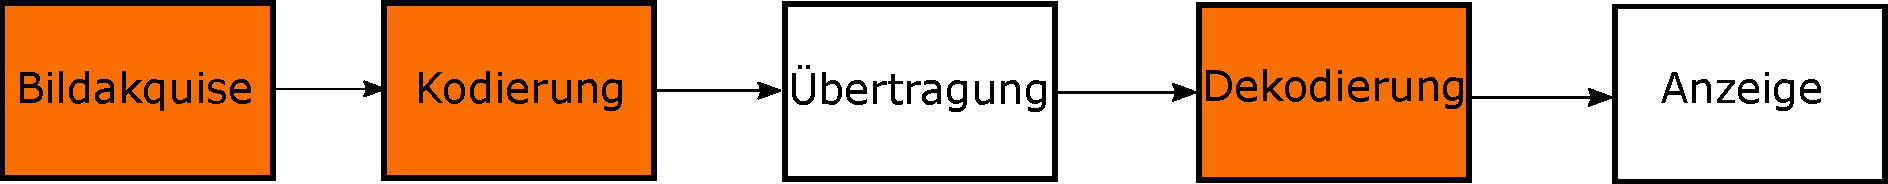
\includegraphics[width=1\textwidth]{Bilder/BildakquiseUndDatenaufbereitung/Bildakquise_schritte.pdf}
	\caption{Prozessschitte zur Anzeige der der Bilddaten auf dem Zielgerät. Die in diesem Kapitel behandelten Schritte sind farbig markiert.}
	\label{fig:Bildakquise_schritte}
\end{figure}

Im vorliegenden Kapitel wird primär auf die Schritte \textit{Bildakquise}, \textit{Kodierung} sowie \textit{Dekodierung} eingegangen, da die Implementierungen dieser Funktionalitäten direkt voneinander abhängen und somit nicht getrennt betrachtet werden können. Die Datenübertragung und Anzeige der Bilddaten bleiben hingegen unbeeinflusst von den genannten Prozessschritten und werden somit gesondert behandelt.\\

\section{Bildakquise}
Der Prozesschritt der Bildakquise beinhaltet die Ermittlung der Bilddaten von dem Quellgerät. Dabei können, je nach vorhandener Hard- und Softwarekonfiguration verschiedene Ansätze verfolgt werden.\\
\\
Ein möglicher Ansatz ist die Verwendung eines Hardwareadapters (\glqq FrameGrabber\grqq), welcher die Videosignale des Quellgerätes über dessen Videoausgang entgegennimmt und über eine Datenschnittstelle einem verarbeitenden Gerät zur Verfügung stellt. Ein Vorteil dieser Vorgehensweise ist die Simplizität in Bezug auf das Quellgerät. Da das Videosignal über bereits vorhandene, standardisierte Schnittstellen übertragen wird, muss keine Veränderung an der Software des Gerätes vorgenommen werden.\\
Im Gegenzug dazu wird jedoch ein weiteres Gerät, welches die Bilddaten entgegennimmt und verarbeitet, benötigt. Damit steigt die Gesamtkomplexität des Systems erheblich an, da statt einem Quell- und einem Zielgerät nunmehr ein Quellgerät, ein Zwischengerät zur Verarbeitung und ein Zielgerät benötigt werden.\\

\begin{figure}[h]
	\centering
	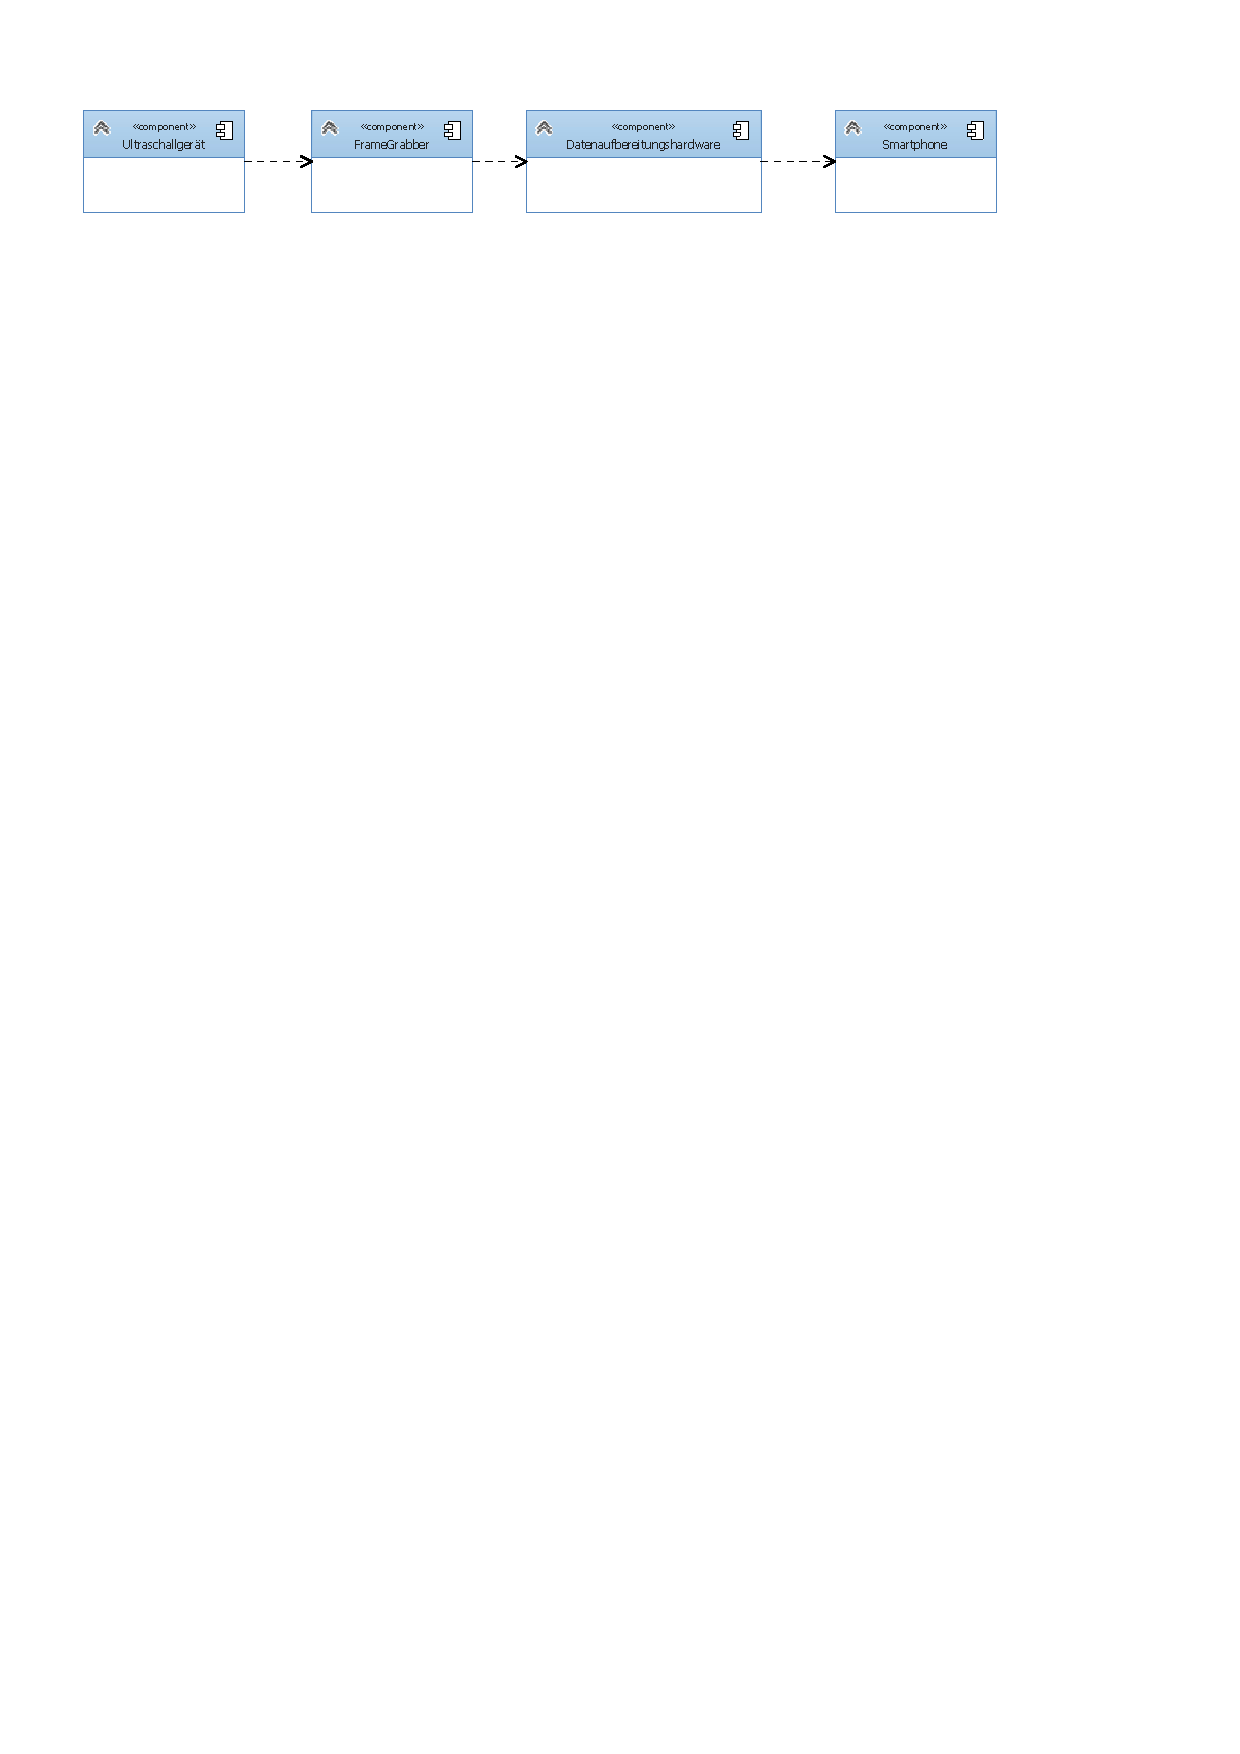
\includegraphics[width=1\textwidth]{Bilder/BildakquiseUndDatenaufbereitung/Bildakquise_ansatz1.pdf}
	\caption{Bildakquise mittels eines FrameGrabbers}
	\label{fig:Bildakquise_ansatz1}
\end{figure}

~\\
Statt der Nutzung eines FrameGrabbers zur Aufnahme der Bilddaten kann auch eine Software, welche die Daten direkt auf dem Ultraschallgerät  aufnimmt und aufbereitet, genutzt werden. Hierzu muss jedoch direkter Zugriff auf das Betriebssystem des Ultraschallgerätes erlangt werden, was sich bei proprietären, geschlossenen Systemen schwierig gestalten kann. Des Weiteren muss die Systemleistung des Quellgerätes ausreichen, um neben der eigentlichen Bildverarbeitung, welche für die Aufnahme des Ultraschallbildes durchgeführt wird, auch noch die Bildakquise und Datenaufbereitung durchzuführen.\\
Der Vorteil dieses Ansatzes im Vergleich zur Nutzung eines FrameGrabbers ist der Wegfall von zwei Hardwarekomponenten im Gesamtsystem: Der FrameGrabber und die Hardware zur Zwischenverarbeitung entfallen, da die entsprechenden Arbeitsschritte direkt auf dem Ultraschallgerät durchgeführt werden können.

\section{Kodierung}
Bei der Kodierung werden die zuvor aufgenommen Bilddaten aufbereitet, um die Übertragung über einen beliebigen Datenkanal zu erleichtern. Dies ist vor allem notwendig, da die Datenmenge der unbehandelten Bilddaten zu hoch für eine Übertragung mittels eines kabellosen Mediums ist.  Wird die Framerate\footnote{Framerate bezeichnet die Anzahl der angezeigten Bilder pro Sekunde} auf 30 FPS\footnote{Frames per second - Bilder pro Sekunde}, die Bildauflösung auf $1024*768$ Pixel und die Farbtiefe auf drei Bytes pro Pixel festgelegt, ergibt sich eine erforderliche Datenrate von
\begin{equation}
D_r=1024*768*3*30=67.5 MByte/s.
\end{equation}
Wenn als Übertragungsmedium WLAN genutzt wird und der 802.11ac\footcite{WIFIStandard} Standard vorausgesetzt werden kann, ist bei einer üblichen Kanalbreite von 20 MHz eine maximale Übertragunsgrate von $96.3 Mbit/s$ oder $12 MByte/s$ möglich. Folglich können die Daten nicht ohne vorherige Kompression übertragen werden.

\section{Dekodierung}
Die Dekodierung rekonstruiert aus dem übertragenen Datenstrom die ursprünglichen Frames und gibt sie an zur Weiterverarbeitung und Anzeige frei. Dieser Prozessschritt wird auf dem Smartphone durchgeführt, da er erst nach der Datenübertragung stattfinden kann.

\section{Implementierung mit FFmpeg}
Im Verlaufe des Projektes wurden zwei verschiedene Ansätze implementiert und getestet. Bei dem ersten Ansatz wurden die Schritte der Bildakquise und Kodierung unter Zuhilfenahme der FFmpeg-Bibliothek\footcite{FFmpeg} realisiert, während zur Dekodierung unter anderem die Android MediaCodec Api\footcite{AndroidMediaCodec} genutzt wurde.\\
Die FFmpeg-Bibliothek bietet die Möglichkeit, über einen Kommandozeilenbefehl den aktuellen Bildschirminhalt als Videostream abzugreifen sowie die entstehenden Daten mit diversen Videocodecs zu kodieren. Der resultierende Datenstrom kann über die unter Linux vorhandene Pipe-Funktionalität in einen gesonderten Prozess umgeleitet werden, welcher die Übertragung bewerkstelligt.\\
\begin{figure}[H]
	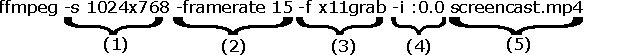
\includegraphics[width=1\textwidth]{Bilder/BildakquiseUndDatenaufbereitung/ffmpeg_befehl1.pdf}
	\caption{FFmpeg-Befehl zur Aufnahme und Speicherung des Bildschirminhaltes.}
	\label{fig:FFmpeg_befehl1}
\end{figure}

Ein beispielhafter FFmpeg-Befehl, welcher den Bildschirminhalt aufnimmt und in einer Datei abspeichert, kann Abbildung \ref{fig:FFmpeg_befehl1} entnommen werden. Es werden fünf Parameter angegeben, welche zur Ausführung des Befehls notwendig sind:
\begin{enumerate} 
	\item Der Schalter \textit{-s} legt die Auflösung des Quellmaterials fest. 
	\item Der Schalter \textit{-framerate} legt die Framerate fest.
	\item Der Schalter \textit{-f} legt die Videoquelle fest. Im gegebenen Fall ist die Quelle  das \textit{x11grab}-Device, welches unter Linux den Bildschirminhalt aufnimmt.
	\item Der Schalter \textit{-i} legt den Abschnitt, welcher abgefilmt werden soll, fest. Da der gesamte Bildschirm des Ultraschallgerätes aufgenommen werden soll, wird die linke obere Ecke des Bildschirms als Startpunkt angegeben.
	\item Die letzte Option gibt den Namen der Ausgabedatei an. 
\end{enumerate}

\subsection{Auswahl eines Videocodecs}
Die FFmpeg-Bibliothek unterstützt eine große Anzahl unterschiedlicher Videocodecs zur Kompression des Quellmaterials. Da die Dekodierung des Datenstroms auf dem Smartphone möglichst schnell und ressourcenschonend ablaufen soll, bietet es sich an, die vorhandene Hardwareunterstützung des Gerätes zu Nutzen. Hierbei wird die Dekodierung von einem dedizierten Hardwareschaltkreis durchgeführt, was die CPU des Smartphones entlastet und den Prozess deutlich beschleunigt. Die Anforderung der Hardwarebeschleunigung schränkt die Auswahl der möglichen Videocodecs deutlich ein.\\
Nach diversen Tests mit dem zur Verfügung stehenden Smartphone fiel die Wahl auf den H.264\footcite{H264} Videocodec, da dieser sowohl eine ausreichende Kompressionsrate bietet, als auch von der FFmpeg-Bibliothek sowie dem Smartphone-Decoder unterstützt wird.\\
Als Pixelformat wurde das NV12-Format\footcite{NV12} gewählt, da dieses die beste Unterstützung seitens des Smartphones aufwies.\\

\begin{lstlisting}[caption=Endgültiger FFmpeg-Konsolenbefehl zur Videoaufnahme, label=lst:ffmpeg_befehl, language=Java]
ffmpeg -s 1024x768 -framerate 15 -f x11grab -i :0.0 -pix_fmt nv12 
-c:v libx264 -x264opts keyint=10:min-keyint=10:scenecut=-1 
-b:v 6000000 -f h264 pipe:| videostream.bin
\end{lstlisting}

~\\
Dem Listing \ref{lst:ffmpeg_befehl} ist der endgültige Befehl zur Aufnahme des Live-Videos zu entnehmen. Zusätzlich zu dem zuvor dargestellten Befehl in Abbildung \ref{fig:FFmpeg_befehl1} wurden noch Schalter für das Pixelformat, den Videocodec sowie dessen Konfiguration angegeben. Über den \textit{pipe}-Ausdruck wird der gesamte Datenstrom umgeleitet und kann somit von einer beliebigen Software über den Standardinput ausgelesen und übertragen werden.

\subsection{Nutzung des MediaCodec}
Zur Dekodierung der Daten kann die Android MediaCodec Api genutzt werden. Diese stellt sicher dass die Verarbeitung der komprimierten Videodaten hardwarebeschleunigt über den dedizierten Schaltkreis des Gerätes stattfindet. \\

\begin{figure}[h]
	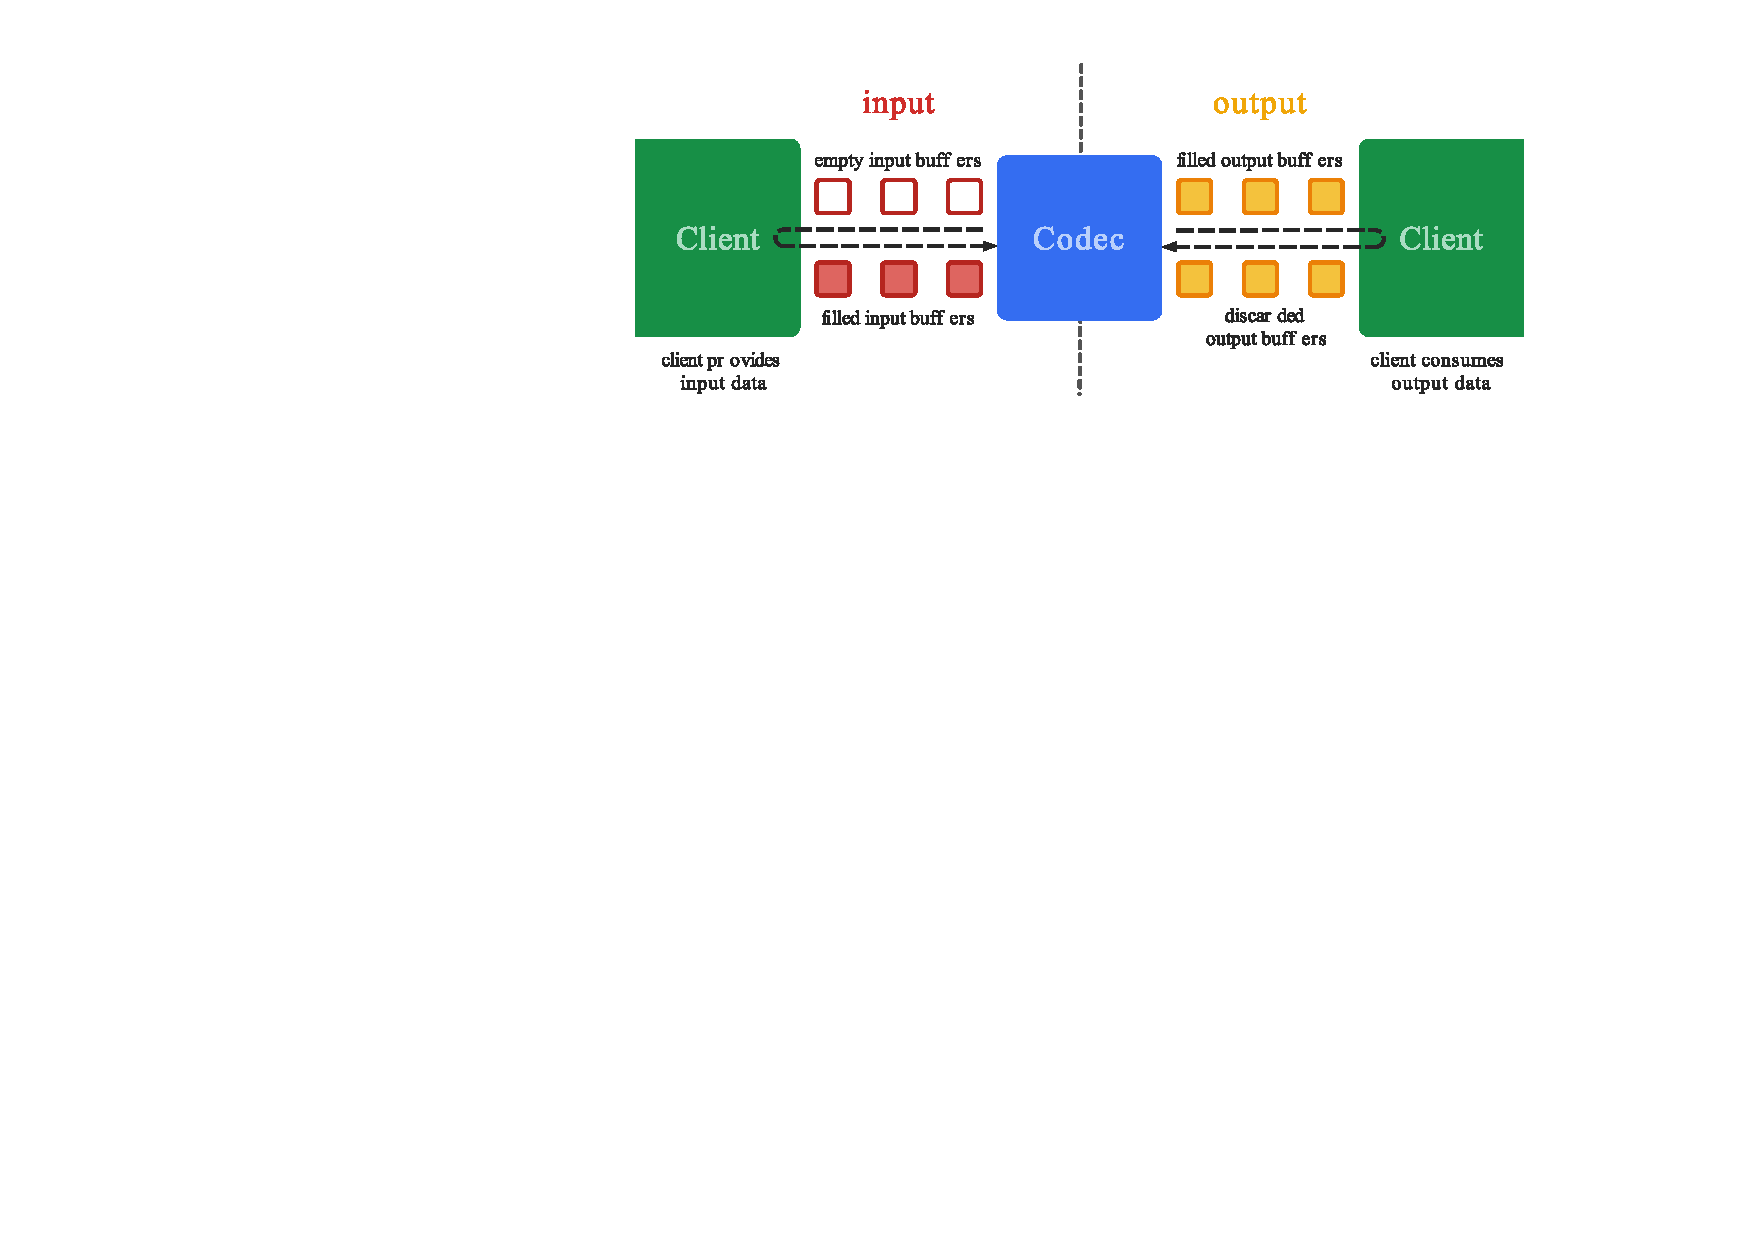
\includegraphics{Bilder/BildakquiseUndDatenaufbereitung/mediacodec.pdf}
	\caption[Nutzung der Android MediaCdec Api]{Nutzung der Android MediaCodec Api\footnotemark}
	\label{fig:media_codec}
\end{figure}
\footnotetext{\cite{AndroidMediaCodec}}
Die MediaCodec Api wird genutzt, indem die komprimierten Rohdaten Paketweise über Eingabepuffer an den Codec übertragen werden. Nach der Dekodierung werden die resultierenden Frames über die vom Codec zur Verfügung gestellten Ausgabepuffer ausgelesen und angezeigt.\\
Da die Daten als kontinuierlicher Datenstrom an das Smartphone gesendet werden, müssen sie vor der Übergabe an den MediaCodec in einzelne Pakete eingeteilt werden. Dabei ist es wichtig, dass die Pakete die erwartete Struktur und den erwarteten Inhalt aufweisen. Diese Eigenschaften sind von dem verwendeten Codec abhängig.\\
 In der vorliegenden Implementierung wurde als Übertragungsformat für die Rohdaten das Annex-B Format genutzt, bei welchem die Daten in sogenannte NALUs\footnote{Network Access Layer Unit} eingeteilt werden. Für den H.264 Codec entspricht somit ein Paket einer NALU.\\
\begin{figure}[H]
	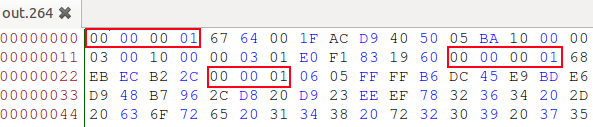
\includegraphics{Bilder/BildakquiseUndDatenaufbereitung/NALUs.png}
	\caption{Rohdaten mit Delimitern.}
	\label{fig:nalus_delimiter}
\end{figure}
In dem Datenstrom sind die einzelnen NALUs durch eine festgelegte Bitfolge ("`Delimiter") voneinander getrennt. Im Hexadezimalsystem kann der Delimiter als \textit{00 00 00 01} oder alternativ mit einer Länge von drei Bytes als \textit{00 00 01} dargestellt werden. Beide Varianten sind dem Annex-B Standard zufolge gültige Delimiter.\\

\subsection{Verarbeitung des Datenstroms}
Zur korrekten Nutzung des MediaCodec muss der Rohdatenstrom also anhand der Delimiter in Echtzeit in einzelne NALUs aufgeteilt werden, welche darauffolgend in die Eingabepuffer des Codec gefüllt werden können. In der Implementierung sind dafür zwei Interfaces vorgesehen.\\
\clearpage
\textbf{INalUExtractor}\\
Das INalUExtractor-Interface stellt die Funktion \textit{extractNalUs()} zur Verfügung, welcher ein Byte-Array und die länge der enthaltenen Daten in Bytes übergeben werden kann. Das Ergebnis der Methode ist eine Liste von Byte-Arrays, die jeweils einegültige NALU enthalten und direkt dem MediaCodec-Eingabepuffer übergeben werden können. Sollten in den Übergebenen Daten unvollständige NALUs vorhanden sein (bspw. wenn der gelesene Block des Datenstroms nicht mit einem vollständigen Delimiter endet), werden diese Daten vorgehalten und beim nächsten Aufruf der Methode verarbeitet.\\
Somit ermöglicht eine gültige Implementierung des Interfaces die kontinuierliche Übergabe von beliebig langen Datenblöcken, welche dann in gültige NALUs aufgeteilt werden.\\
\begin{lstlisting}[caption=Definition des INaluUExtractor-Interface, label=lst:i_nalu_extractor, language=Java]
public interface INalUExtractor
{
    List<byte[]> extractNalUs(byte[] data, int length);
}
\end{lstlisting}
~\\
\\
\textbf{INalUSplitter}\\
Das INalUSplitter-Interface wird von der Implementierung des INalUExtractor-Interfaces genutzt, um einen Datenblock zu einem \textit{NalUSplitResult} zu verarbeiten. Es definiert die Methode \textit{splitBlock()} welche ein Byte-Array sowie die Länge der enthaltenen Daten erwartet und das Ergebis der Operation als \textit{NalUSplitResult} zurück gibt.

\begin{lstlisting}[caption=Definition der NalUSplitResult-Klasse, label=lst:nalu_split_result, language=Java]
public class NalUSplitResult
{
    private byte[] partialStartPart;
    private List<byte[]> completeNalUs;
    private byte[] partialEndPart;
    
    // Getter und Setter...
}
\end{lstlisting}

Ein \textit{NalUSplitResult} repräsentiert einen Datenblock, aufgeteilt in drei Komponenten. Das Feld \textit{partialStartPart} enthält die Bytes einer unvollständigen NALU zu beginn des Datenblockes. Eine solche NALU entsteht, wenn der vorherige Datenblock nicht mit einer vollständigen NALU endet und somit der aktuelle Datenblock nicht mit einem gültigen Delimiter beginnt.\\
Das Feld \textit{completeNalUs} enthält alle vollständigen, gültigen NALUs, die in dem übergebenen Datenblock vorhanden sind. Das Feld \textit{partialEndPart} enthält die Bytes, welche am Ende eines Datenblockes liegen aber nicht eindeutig eine vollständige NALU repräsentieren.\\
Die NalUSplitResult-Instanzen, welche für die Datenblöcke generiert werden, werden vom \textit{NalUExtractor} genutzt, um die unvollständigen Datenblöcke zusammenzuführen und einen kontinuierlichen Strom gültiger NALUs zu erzeugen.\\
\begin{lstlisting}[caption=Definition des INaluUSplitter-Interface, label=lst:i_nalu_splitter, language=Java]
public interface INalUSplitter 
{
    NalUSplitResult splitBlock(byte[] block, int length);
}
\end{lstlisting}

\subsection{Konfiguration des MediaCodec}
Zusätzlich zu den Datenpaketen, welche von der MediaCodec-Api erwartet werden, müssen noch weitere Konfigurationen zur erfolgreichen Nutzung des Codecs vorgenommen werden. Dazu gehören die Angabe des MIME-type des vorhandenen Videoformates und das Setzen der SPS\footnote{Sequence Parameter Set, enthält Informationen über den Aufbau des Videostreams} und PPS\footnote{Picture Parameter Set, enthält Informationen über die Konfiguration der einzelnen Frames.} Felder des Codecs.\\
 Diese Konfigurationen werden vor dem Start des Decoding-Prozesses vorgenommen. Die Datenübergabe an den Eingabepuffer und das Auslesen der Daten aus dem Ausgabepuffer erfolgt schließlich über Callback-Funktionen, welche für den Codec registriert werden müssen. \\
\\
Die Bytefolgen für die SPS- und PPS-Felder können ermittelt werden, indem gewisse NALUs eines Streams mit der gewünschten Konfiguration im Annex-B Format manuell analysiert werden. Jede NALU hat einen Typen, welcher über das erste Byte nach dem Delimiter festgelegt wird. Kommt in dem Stream eine NALU mit der Bitfolge \textit{0x67} (in Hexadezimaldarstellung) vor, handelt es sich um das SPS-Feld. Die Bitfolge \textit{0x68} signalisiert das PPS-Feld. 

\begin{lstlisting}[caption=Konfiguration des MediaCodec, label=lst:config_media_codec, language=Java]

private static final String MIME_TYPE = "video/avc";
private static final int WIDTH = 1280;
private static final int HEIGHT = 720;

private void configureCodec()
{
	codec = MediaCodec.createDecoderByType(MIME_TYPE);
	MediaFormat format = MediaFormat.createVideoFormat(MIME_TYPE, WIDTH, HEIGHT);
	byte[] sps = {  //...SPS-Bytes...};
	byte[] pps = { //...PPS-Bytes...};
	format.setByteBuffer("csd-0", ByteBuffer.wrap(sps));
	format.setByteBuffer("csd-1", ByteBuffer.wrap(pps));
	codec.configure(format, null, null, 0);
	//... Registrierung der Callbacks...
	codec.start();
}
\end{lstlisting}

\subsection{Performance und Funktionalität}
Die Implementierung mit den vorgestellten Methoden und Ansätzen funktionierte auf den Testgeräten nur eingeschränkt. Die Performance war zwar, sowohl auf dem Ultraschallgerät als auch auf dem Smartphone, sehr zufriedenstellend und das Datenaufkommen minimal, die Latenz der Gesamtlösung lag jedoch bei mehr als 2000 mS. Eine Echtzeitanwendung ist damit nur sehr eingeschränkt möglich, da Veränderungen des Ultraschallbildes erst mit einer großen Verzögerungen auf dem Smartphone angezeigt werden.\\
Die Latenz konnte auch durch Die Nutzung anderer alternativer Übertragungsformen und Videocodecs nur unzureichend verringert werden, da alleine das \textit{x11grab}-Device zur Aufnahme des Bildschirminhaltes eine Latenz von 800 mS erzeugte. \\

\section{Implementierung mit X11Lib und LZ4}
Da die Implementierung mit Hilfe der FFmpeg-Bibliothek eine zu hohe Latenz aufwies, musste eine Alternative gefunden werden. Bei der Konzeption stand, neben den schon zuvor ermittelten Anforderungen an die Performance und das Datenaufkommen, vor allem die Latenz im Mittelpunkt.\\ Es musste also für jeden Prozessschritt eine Implementierung geschaffen werden, welche innerhalb weniger Millisekunden ausgeführt werden kann um in der Summe auf eine Gesamtdauer von weniger als 200 mS zu kommen. 

\subsection{Bildakquise mit X11Lib}
X11Lib ist eine C++-Bibliothek, welche den direkten Zugriff auf Bilddaten des Linux-Grafiksystems ermöglicht. Zur Aufnahme des aktuell angezeigten Bildschirminhaltes kann die Funktion \textit{XGetImage()} genutzt werden, welche die Bilddaten in einem zuvor festgelegten Format in ein \textit{char-Array} abspeichert.\\
Ein Vorteil dieser Funktion ist die hohe Performance. Die Bildaufnahme dauerte auf dem Testgerät lediglich acht Millisekunden, wodurch für die weiteren Schritte noch 192 mS verbleiben.

\begin{lstlisting}[caption=Bildaufnahme mittels X11Lib, label=lst:capture_x11lib, language=C++]
display = XOpenDisplay(NULL);
root = DefaultRootWindow(display);
XWindowAttributes gwa;
XGetWindowAttributes(display, root, &gwa);
width = 1024, height=768;

image = XGetImage(display,root, 0,0 , width,height,AllPlanes, ZPixmap);
\end{lstlisting}
~\\
Das Bild wird im ARGB8888-Format abgespeichert, wobei jeder Kanal ein Byte belegt. Ein Pixel besteht also aus vier aufeinanderfolgenden Bytes.

\subsection{Datenreduktion}
Da für die Aufnahme des Bildschirminhaltes der Alphakanal nicht benötigt wird, muss dieser nicht an das Smartphone übertragen werden. Des Weiteren wird auf dem Smartphone das RGB565-Format genutzt, welches pro Pixel nur zwei Bytes benötigt. Um die übertragenen Datenmenge zu reduzieren, erfolgt die Umwandlung des Pixelformates auf dem Ultraschallgerät, wodurch die unkomprimierten Rohdaten nur noch zwei Bytes pro Pixel in Anspruch nehmen.\\
\\
Da die Umwandlung Pixelweise und damit sehr häufig erfolgt, wurde bei der Implementierung großer Wert auf die Performance der einzelnen Operationen gelegt. Die Konvertierung besteht aus den folgenden Schritten:
\begin{enumerate}
\item{Rechne den Wertebereich für den Rotanteil von acht Bits auf fünf Bits um}
\item{Schreibe den neuen Rotanteil in die fünf MSB\footnote{Most significant Bits} des ersten Zielbytes}
\item{Rechne den Wertebereich des Grünanteils von acht Bits auf sechs Bits um}
\item{Schreibe die drei MSB des neuen Grünanteils in die drei LSB\footnote{Least significant Bits} des ersten Zielbytes}
\item{Schreibe die drei LSB des neuen Grünanteils in die drei MSB des zweiten Zielbytes}
\item{Rechne den Wertebereich des Blauanteils von acht Bits auf fünf Bits um}
\item{Schreibe den neuen Blauanteil in die fünf LSB des zweiten Zielbytes}
\end{enumerate}

Da primitive Bitoperationen deutlich schneller ausgeführt werden können als andere mathematische Operationen, beschränkt sich die C++-Implementierung der Konvertierung auf eine Kombination von Bitshifts und Bitweisen UND-Verknüpfungen. Die Bitshifts ermöglichen die Verkleinerung des Wertebereiches durch das Abschneiden weniger signifikanter Bits, während die UND-Verknüpfungen das Löschen unerwünschter Bits in den Zielbytes bewerkstelligen.\\
Die gesamte Umwandlung eines Frames mit den Maßen von $1024*768$ Pixeln benötigt insgesamt fünf Millisekunden, womit die Gesamtdauerdauer der Operationen auf 13 Millisekunden steigt.

\begin{lstlisting}[caption=Umwandlung des Pixelformates, label=lst:rgb_conversion, language=C++]
for(int row = 0; row < height; row++)
{
        for(int col = 0; col < width; col++)
        {
            srcStartIdx = row*width*4+col*4;
            destStartIdx = row*width*2+col*2;

            // Convert to RGB565
            rgb565Data[destStartIdx] =
             ((data[srcStartIdx+1] << 3) & 0x00E0)|((data[srcStartIdx] >> 3) & 0x001F);
            rgb565Data[destStartIdx+1] = 
             (data[srcStartIdx+2] & 0x00F8)|((data[srcStartIdx+1] >> 5) & 0x0007);
        }
    }
\end{lstlisting}

\subsection{Kompression}
Um die zu übertragende Datenmenge weiter zu reduzieren, wurde das LZ4-Verfahren\footcite{LZ4} zur Kompression der Bilddaten verwendet. Bei dem LZ4-Verfahren handelt es sich um eine Verlustfreie Kompression, welche für hohe Kompressions- und Dekompressionsgeschwindigkeiten optimiert ist. Dadurch ist es optimal für den gegebenen Einsatzzweck geeignet, da die Datenrate zwar relevant ist, die Latenz jedoch stark von der Vorverarbeitung eingeschränkt wird. Somit muss ein Kompromiss gefunden werden, welcher die Datenmenge reduziert ohne die Verarbeitungsdauer stark zu beeinflussen. \\
Die unkomprimierte Größe eines Frames mit den Abmessungen $1024*768$ beträgt
\begin{equation}
N_1=1024*768*2=1572864 Bytes
\end{equation}.
Die C++-Implementierung des LZ4-Algorithmus verringerte das Datenaufkommen zu einer Größe von $64252 Bytes$. Damit beträgt die Kompressionsrate 
\begin{equation}
C_R=1572864/64252=24.48
\end{equation}
und die Redundanz
\begin{equation}
R_D=1-1/C_R=0.96
\end{equation}
Die Kompression dauerte auf dem Testgerät elf Millisekunden, womit der gesamte Vorgang vor der Übertragung 23 mS in Anspruch nimmt.

\begin{lstlisting}[caption=Kompression der Rohdaten, label=lst:compression, language=C++]
// Komprimiert die Daten aus dem Quellarray "rgb565Data" in das Zielarray "compressedFile"
// und speichert die Laenge des komprimierten Arrays in "compressedBytes"
compressedBytes = LZ4_compress_default(
	rgb565Data, compressedFile, rgb565DataSize, 500000);
\end{lstlisting}

\subsection{Verarbeitung auf dem Smartphone}
Zur Anzeige der Bilddaten auf dem Smartphone werden die komprimierten Daten mit Hilfe einer Java-Portierung der LZ4-Bibliothek\footcite{JPounzLZ4} dekomprimiert und die RGB565-Rohdaten zu einem Android-Bitmap Objekt verarbeitet. Das resultierende Frame kann dann auf der Oberfläche der Smartphone-Anwendung angezeigt werden.

\begin{lstlisting}[caption=Dekompression der Daten, label=lst:decompression, language=Java]
// Erzeuge notwendige Objekte zur Dekomprimierung
LZ4Factory factory = LZ4Factory.safeInstance();
LZ4FastDecompressor decompressor = factory.fastDecompressor();

// Dekomprimiere die Daten
int res = decompressor.decompress(dataBytes, decompressedData, decompressedData.length);

// Wandle die Rohdaten in eine Android Bitmap Objekt um
final Bitmap b = getBitmapFromData(decompressedData, width, height);
\end{lstlisting}

\subsection{Performance und Funktionalität}
Die vorgestellte Implementierung hat gegenüber der FFmpeg-Variante zwei Nachteile: Sowohl die entstehende Datenmenge, als auch die Prozessorlast ist wesentlich höher. Beide Nachteile sind jedoch für den gegebenen Anwendungsfall nicht relevant, da die Prozessorlast sich in den Tests nicht auf die Leistung des Ultraschallgerätes auswirkte und die Kapazitätsreserven des verwendeten Übertragungsmediums die erhöhte Datenrate problemlos abfangen konnten.\\
Im Gegenzug beträgt die Gesamtlatenz des Systems, also die Dauer von der Bildaufnahme auf dem Ultraschallgerät bis zur Bildanzeige auf dem Smartphone, weniger als 200 mS und ist damit um eine Größenordnung geringer als der alternative Ansatz. Die errreichte Framerate liegt zwischen 12 FPS und 30 FPS. Somit werden alle spezifizierten Anforderungen durch die Implementierung zufriedenstellend erfüllt. Zusätzlich ist die vorliegende Lösung, im Gegensatz zum FFmpeg-Basierten Ansatz, komplett verlustfrei und eröffnet damit noch weitere Möglichkeiten zur pixelgenauen Verarbeitung der Ultraschallbilder.

\subsection{Optimierungspotenzial}
Die vorliegende Implementierung kann, gerade in Bezug auf die Kompression, noch weiter Optimiert werden. Der erste Ansatz führt die Kompression für jedes Frame einzeln durch, wobei eine gesamte Dimension, die Zeitdimension, des Videostreams nicht beachtet wird.\\
Der vorliegende Anwendungsfall hat zwei ungewöhnliche Eigenschaften, die die Zeitdimension für die Kompression relevant werden lassen:
\begin{enumerate}
\item{Es werden digitale Bilder abgefilmt. Damit liegt keinerlei Bildrauschen vor.}
\item{Die übertragenen Frames sind identisch (bei stillstehendem Bild) oder haben zumindest große, identische Bereiche.}
\end{enumerate}

Diese Eigenschaften können genutzt werden, um die Kompressionsleistung noch einmal zu steigern, indem statt eines kompletten Frames nur noch die Differenz zu dem vorherigen Frame übertragen wird. Dadurch werden identische Bereiche zu Null (da es kein Bildrauschen gibt). Daten, welche eine große Anzahl aufeinanderfolgender Nullen enthalten, können wesentlich besser komprimiert werden. In vorläufigen Tests mit der LZ4-Bibliothek betrug die Größe eines komprimierten Differenzbildes nur noch ein Fünftel der Größe eines komprimierten Frames.\\
In der aktuellen Implementierung wurde dieser Ansatz nicht weiter verfolgt, da die Kompressionsleistung bereits ausreichte und alle Anforderungen erfüllt wurden. Für zukünftige Einsatzzwecke könnte eine weitere Optimierung des Systems jedoch durchaus erhebliche Vorteile bieten.

